% Options for packages loaded elsewhere
\PassOptionsToPackage{unicode}{hyperref}
\PassOptionsToPackage{hyphens}{url}
%
\documentclass[
]{book}
\usepackage{amsmath,amssymb}
\usepackage{lmodern}
\usepackage{iftex}
\ifPDFTeX
  \usepackage[T1]{fontenc}
  \usepackage[utf8]{inputenc}
  \usepackage{textcomp} % provide euro and other symbols
\else % if luatex or xetex
  \usepackage{unicode-math}
  \defaultfontfeatures{Scale=MatchLowercase}
  \defaultfontfeatures[\rmfamily]{Ligatures=TeX,Scale=1}
\fi
% Use upquote if available, for straight quotes in verbatim environments
\IfFileExists{upquote.sty}{\usepackage{upquote}}{}
\IfFileExists{microtype.sty}{% use microtype if available
  \usepackage[]{microtype}
  \UseMicrotypeSet[protrusion]{basicmath} % disable protrusion for tt fonts
}{}
\makeatletter
\@ifundefined{KOMAClassName}{% if non-KOMA class
  \IfFileExists{parskip.sty}{%
    \usepackage{parskip}
  }{% else
    \setlength{\parindent}{0pt}
    \setlength{\parskip}{6pt plus 2pt minus 1pt}}
}{% if KOMA class
  \KOMAoptions{parskip=half}}
\makeatother
\usepackage{xcolor}
\IfFileExists{xurl.sty}{\usepackage{xurl}}{} % add URL line breaks if available
\IfFileExists{bookmark.sty}{\usepackage{bookmark}}{\usepackage{hyperref}}
\hypersetup{
  pdftitle={Data Science \& Machine Learning},
  pdfauthor={Dieter Greipl},
  hidelinks,
  pdfcreator={LaTeX via pandoc}}
\urlstyle{same} % disable monospaced font for URLs
\usepackage{color}
\usepackage{fancyvrb}
\newcommand{\VerbBar}{|}
\newcommand{\VERB}{\Verb[commandchars=\\\{\}]}
\DefineVerbatimEnvironment{Highlighting}{Verbatim}{commandchars=\\\{\}}
% Add ',fontsize=\small' for more characters per line
\usepackage{framed}
\definecolor{shadecolor}{RGB}{248,248,248}
\newenvironment{Shaded}{\begin{snugshade}}{\end{snugshade}}
\newcommand{\AlertTok}[1]{\textcolor[rgb]{0.94,0.16,0.16}{#1}}
\newcommand{\AnnotationTok}[1]{\textcolor[rgb]{0.56,0.35,0.01}{\textbf{\textit{#1}}}}
\newcommand{\AttributeTok}[1]{\textcolor[rgb]{0.77,0.63,0.00}{#1}}
\newcommand{\BaseNTok}[1]{\textcolor[rgb]{0.00,0.00,0.81}{#1}}
\newcommand{\BuiltInTok}[1]{#1}
\newcommand{\CharTok}[1]{\textcolor[rgb]{0.31,0.60,0.02}{#1}}
\newcommand{\CommentTok}[1]{\textcolor[rgb]{0.56,0.35,0.01}{\textit{#1}}}
\newcommand{\CommentVarTok}[1]{\textcolor[rgb]{0.56,0.35,0.01}{\textbf{\textit{#1}}}}
\newcommand{\ConstantTok}[1]{\textcolor[rgb]{0.00,0.00,0.00}{#1}}
\newcommand{\ControlFlowTok}[1]{\textcolor[rgb]{0.13,0.29,0.53}{\textbf{#1}}}
\newcommand{\DataTypeTok}[1]{\textcolor[rgb]{0.13,0.29,0.53}{#1}}
\newcommand{\DecValTok}[1]{\textcolor[rgb]{0.00,0.00,0.81}{#1}}
\newcommand{\DocumentationTok}[1]{\textcolor[rgb]{0.56,0.35,0.01}{\textbf{\textit{#1}}}}
\newcommand{\ErrorTok}[1]{\textcolor[rgb]{0.64,0.00,0.00}{\textbf{#1}}}
\newcommand{\ExtensionTok}[1]{#1}
\newcommand{\FloatTok}[1]{\textcolor[rgb]{0.00,0.00,0.81}{#1}}
\newcommand{\FunctionTok}[1]{\textcolor[rgb]{0.00,0.00,0.00}{#1}}
\newcommand{\ImportTok}[1]{#1}
\newcommand{\InformationTok}[1]{\textcolor[rgb]{0.56,0.35,0.01}{\textbf{\textit{#1}}}}
\newcommand{\KeywordTok}[1]{\textcolor[rgb]{0.13,0.29,0.53}{\textbf{#1}}}
\newcommand{\NormalTok}[1]{#1}
\newcommand{\OperatorTok}[1]{\textcolor[rgb]{0.81,0.36,0.00}{\textbf{#1}}}
\newcommand{\OtherTok}[1]{\textcolor[rgb]{0.56,0.35,0.01}{#1}}
\newcommand{\PreprocessorTok}[1]{\textcolor[rgb]{0.56,0.35,0.01}{\textit{#1}}}
\newcommand{\RegionMarkerTok}[1]{#1}
\newcommand{\SpecialCharTok}[1]{\textcolor[rgb]{0.00,0.00,0.00}{#1}}
\newcommand{\SpecialStringTok}[1]{\textcolor[rgb]{0.31,0.60,0.02}{#1}}
\newcommand{\StringTok}[1]{\textcolor[rgb]{0.31,0.60,0.02}{#1}}
\newcommand{\VariableTok}[1]{\textcolor[rgb]{0.00,0.00,0.00}{#1}}
\newcommand{\VerbatimStringTok}[1]{\textcolor[rgb]{0.31,0.60,0.02}{#1}}
\newcommand{\WarningTok}[1]{\textcolor[rgb]{0.56,0.35,0.01}{\textbf{\textit{#1}}}}
\usepackage{longtable,booktabs,array}
\usepackage{calc} % for calculating minipage widths
% Correct order of tables after \paragraph or \subparagraph
\usepackage{etoolbox}
\makeatletter
\patchcmd\longtable{\par}{\if@noskipsec\mbox{}\fi\par}{}{}
\makeatother
% Allow footnotes in longtable head/foot
\IfFileExists{footnotehyper.sty}{\usepackage{footnotehyper}}{\usepackage{footnote}}
\makesavenoteenv{longtable}
\usepackage{graphicx}
\makeatletter
\def\maxwidth{\ifdim\Gin@nat@width>\linewidth\linewidth\else\Gin@nat@width\fi}
\def\maxheight{\ifdim\Gin@nat@height>\textheight\textheight\else\Gin@nat@height\fi}
\makeatother
% Scale images if necessary, so that they will not overflow the page
% margins by default, and it is still possible to overwrite the defaults
% using explicit options in \includegraphics[width, height, ...]{}
\setkeys{Gin}{width=\maxwidth,height=\maxheight,keepaspectratio}
% Set default figure placement to htbp
\makeatletter
\def\fps@figure{htbp}
\makeatother
\setlength{\emergencystretch}{3em} % prevent overfull lines
\providecommand{\tightlist}{%
  \setlength{\itemsep}{0pt}\setlength{\parskip}{0pt}}
\setcounter{secnumdepth}{5}
\usepackage{booktabs}
\ifLuaTeX
  \usepackage{selnolig}  % disable illegal ligatures
\fi
\usepackage[]{natbib}
\bibliographystyle{apalike}

\title{Data Science \& Machine Learning}
\author{Dieter Greipl}
\date{2022-01-07}

\usepackage{amsthm}
\newtheorem{theorem}{Theorem}[chapter]
\newtheorem{lemma}{Lemma}[chapter]
\newtheorem{corollary}{Corollary}[chapter]
\newtheorem{proposition}{Proposition}[chapter]
\newtheorem{conjecture}{Conjecture}[chapter]
\theoremstyle{definition}
\newtheorem{definition}{Definition}[chapter]
\theoremstyle{definition}
\newtheorem{example}{Example}[chapter]
\theoremstyle{definition}
\newtheorem{exercise}{Exercise}[chapter]
\theoremstyle{definition}
\newtheorem{hypothesis}{Hypothesis}[chapter]
\theoremstyle{remark}
\newtheorem*{remark}{Remark}
\newtheorem*{solution}{Solution}
\begin{document}
\maketitle

{
\setcounter{tocdepth}{1}
\tableofcontents
}
\hypertarget{willkommen}{%
\chapter*{Willkommen}\label{willkommen}}
\addcontentsline{toc}{chapter}{Willkommen}

Dieses Skript entstand (und entsteht) aus meinen Lehrveranstaltungen rund um das Thema \textbf{Data Science \& Machine Learning}. Die Inhalte richten sich an Studierende, die erste Schritte auf das KI -Spielfeld wagen und das Potential von datengetriebenen Lösungsverfahren verstehen wollen.

Insofern richtet sich die Darstellung an Studierende mit vertieftem Interesse an KI, die einen für Studierende angemessenes Vorwissen im Bereich Mathematik mitbringen. Vorkenntnisse im Bereich der Programmierung sind nicht nötig, aber natürlich hilfreich.

Ich habe mich bemüht, zahlreiche Übungsbeispiele und Youtube-Videos einzubauen. Viele Themen lassen sich so besser darstellen. Sofern es Medien im Netz gibt, die die Sachverhalte gut darstellen, werde ich entsprechenden Links einbauen. Der Autor muss ja nicht der Meinung sein, alles besser zu können. Gleichwohl darf dadurch der rote Faden nicht verloren gehen.

\hypertarget{vorbereitungen}{%
\section{Vorbereitungen}\label{vorbereitungen}}

Dieses Skript ist als Unterlage für zahlreichen praktische Übungen mit Python angelegt. Ich werde hierzu \href{https://colab.research.google.com/}{\textbf{Colab-Notebooks}} verwenden. Sie brauchen hierzu ein \textbf{Google-Konto}.

Noch einige Hinweise an Studierende meiner Module:

\begin{itemize}
\tightlist
\item
  Die folgende Youtube-Playlist kann zur Vertiefung einzelner Stoffteile nutzen: \href{https://youtube.com/playlist?list=PLfGN40VwjduJPvtP9QUjC0rjM6-ePT9bg}{Youtube Playlist}
\item
  Wenige Passagen in diesem Skript sind eventuell in englischer Sprache gehalten.
\item
  Dieses Skript

  \begin{itemize}
  \tightlist
  \item
    befindet sich in Teilen im Aufbau, leichte Fehler sind also möglich (und wahrscheinlich - für Hinweise bin ich dankbar)
  \item
    geht nach der Prüfung off-line
  \end{itemize}
\end{itemize}

\hypertarget{tests-spuxe4ter-luxf6schen}{%
\section{Tests (später löschen!)}\label{tests-spuxe4ter-luxf6schen}}

\begin{Shaded}
\begin{Highlighting}[]
\CommentTok{\#Scatterplot}
\ImportTok{import}\NormalTok{ matplotlib.pyplot }\ImportTok{as}\NormalTok{ plt}
\ImportTok{import}\NormalTok{ seaborn }\ImportTok{as}\NormalTok{ sns}

\NormalTok{years }\OperatorTok{=}\NormalTok{ [}\DecValTok{1950}\NormalTok{, }\DecValTok{1960}\NormalTok{, }\DecValTok{1970}\NormalTok{, }\DecValTok{1980}\NormalTok{, }\DecValTok{1990}\NormalTok{, }\DecValTok{2000}\NormalTok{, }\DecValTok{2010}\NormalTok{]}
\NormalTok{gdp }\OperatorTok{=}\NormalTok{ [}\FloatTok{33.2}\NormalTok{, }\FloatTok{543.3}\NormalTok{, }\FloatTok{1075.9}\NormalTok{, }\FloatTok{2862.5}\NormalTok{, }\FloatTok{5979.6}\NormalTok{, }\FloatTok{10289.7}\NormalTok{, }\FloatTok{14958.3}\NormalTok{]}

\NormalTok{sns.}\BuiltInTok{set}\NormalTok{()}
\NormalTok{fig,ax }\OperatorTok{=}\NormalTok{ plt.subplots()}
\NormalTok{ax.set\_title(}\StringTok{"GDP Development"}\NormalTok{) }
\NormalTok{ax.set\_xlabel(}\StringTok{"Years"}\NormalTok{)}
\NormalTok{ax.set\_ylabel(}\StringTok{"GDP"}\NormalTok{)}
\CommentTok{\#ax.set\_aspect(\textquotesingle{}equal\textquotesingle{})}
\CommentTok{\#ax.set\_xlim(0, 50)}
\CommentTok{\#ax.set\_ylim(0, 35)}

\NormalTok{sns.scatterplot(x}\OperatorTok{=}\NormalTok{years, y}\OperatorTok{=}\NormalTok{gdp, color}\OperatorTok{=}\StringTok{"red"}\NormalTok{, label}\OperatorTok{=}\StringTok{"My Label"}\NormalTok{)          }
\CommentTok{\#sns.lineplot(x=years, y=gdp, color="red", label="My Label")            }
\CommentTok{\#sns.barplot(x=years, y=gdp, color="red", label="My Label")  }
\end{Highlighting}
\end{Shaded}

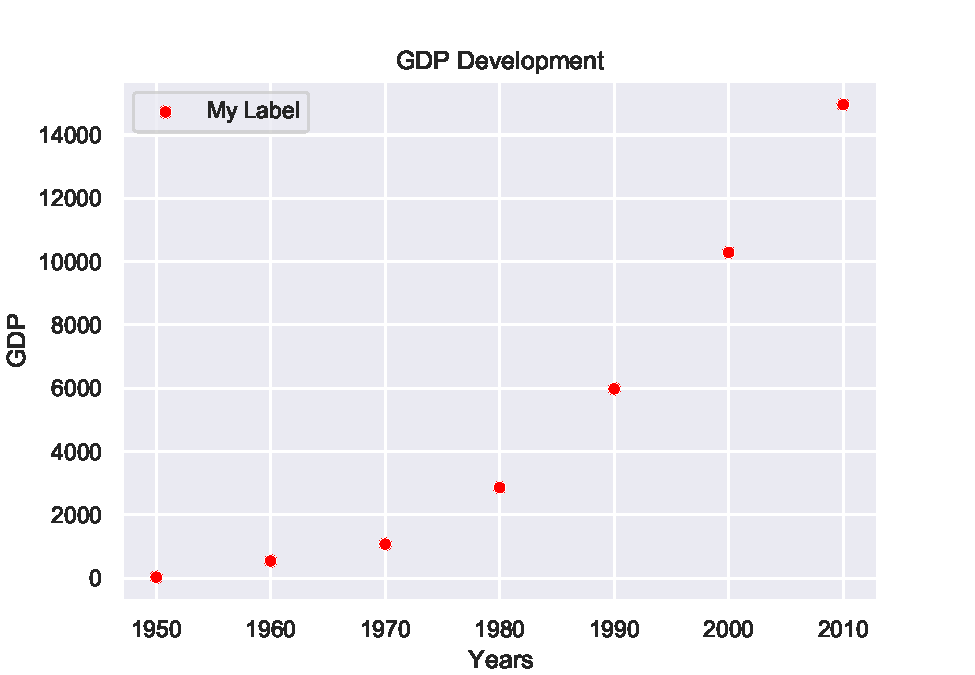
\includegraphics{index_files/figure-latex/unnamed-chunk-1-1.pdf}

\begin{Shaded}
\begin{Highlighting}[]
\ImportTok{import}\NormalTok{ matplotlib.pyplot }\ImportTok{as}\NormalTok{ plt}
\ImportTok{import}\NormalTok{ seaborn }\ImportTok{as}\NormalTok{ sns}
\ImportTok{import}\NormalTok{ numpy }\ImportTok{as}\NormalTok{ np}

\NormalTok{N }\OperatorTok{=} \DecValTok{1000}
\NormalTok{x\_werte }\OperatorTok{=}\NormalTok{ np.random.normal(}\DecValTok{0}\NormalTok{,}\DecValTok{1}\NormalTok{,N)}
\NormalTok{y\_werte }\OperatorTok{=}\NormalTok{ np.random.normal(}\DecValTok{0}\NormalTok{,}\DecValTok{2}\NormalTok{,N)}

\NormalTok{sns.}\BuiltInTok{set}\NormalTok{()}
\NormalTok{fig,ax }\OperatorTok{=}\NormalTok{ plt.subplots(figsize}\OperatorTok{=}\NormalTok{(}\DecValTok{6}\NormalTok{, }\DecValTok{6}\NormalTok{))}
\NormalTok{ax.set\_xlim(}\OperatorTok{{-}}\DecValTok{4}\NormalTok{, }\DecValTok{4}\NormalTok{)}
\CommentTok{\#\textgreater{} ({-}4.0, 4.0)}
\NormalTok{ax.set\_ylim(}\OperatorTok{{-}}\DecValTok{4}\NormalTok{, }\DecValTok{4}\NormalTok{)}
\CommentTok{\#\textgreater{} ({-}4.0, 4.0)}
\NormalTok{ax.set\_aspect(}\StringTok{\textquotesingle{}equal\textquotesingle{}}\NormalTok{)}
\NormalTok{sns.scatterplot(x }\OperatorTok{=}\NormalTok{ x\_werte, y}\OperatorTok{=}\NormalTok{y\_werte)}
\CommentTok{\#print("Wert von N: ", N)}
\end{Highlighting}
\end{Shaded}

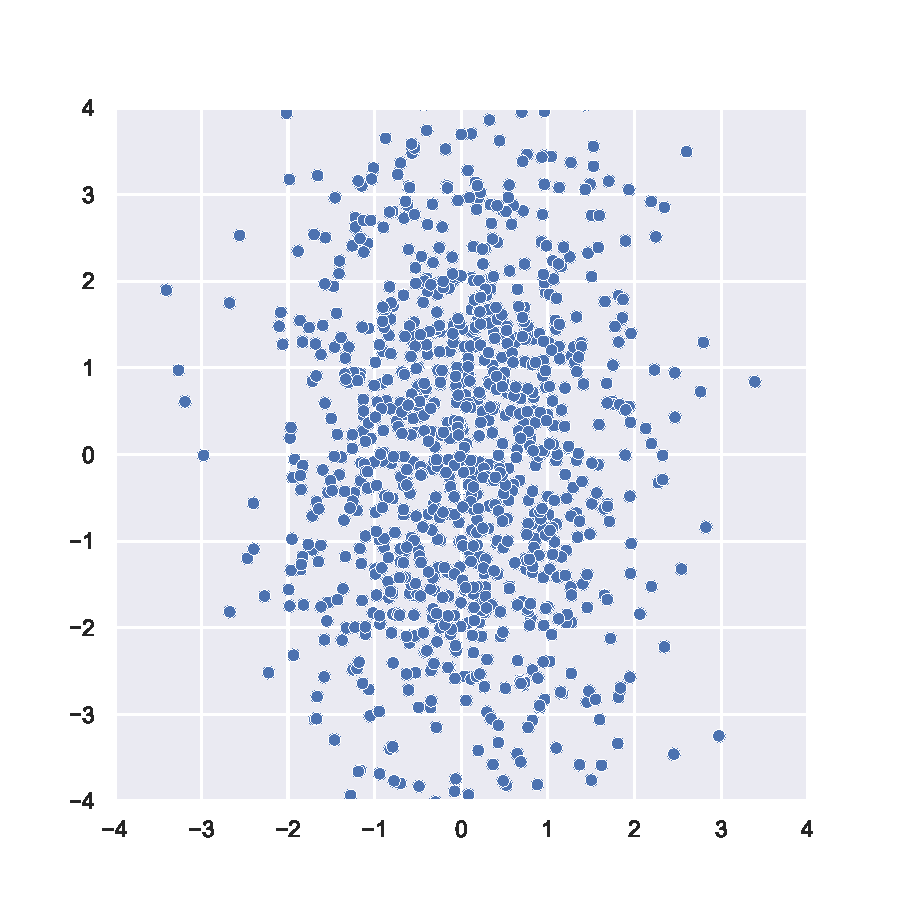
\includegraphics{index_files/figure-latex/unnamed-chunk-2-3.pdf}

Code mit Ausdruck (See \url{https://yihui.org/knitr/options/\#code-evaluation})

\begin{Shaded}
\begin{Highlighting}[]
\NormalTok{x }\OperatorTok{=} \DecValTok{1}
\BuiltInTok{print}\NormalTok{(x)}
\BuiltInTok{print}\NormalTok{(x}\OperatorTok{+}\DecValTok{1}\NormalTok{)}
\CommentTok{\#\textgreater{} 1}
\CommentTok{\#\textgreater{} 2}
\end{Highlighting}
\end{Shaded}

Video

\href{https://youtu.be/Gow7p-rl2HE}{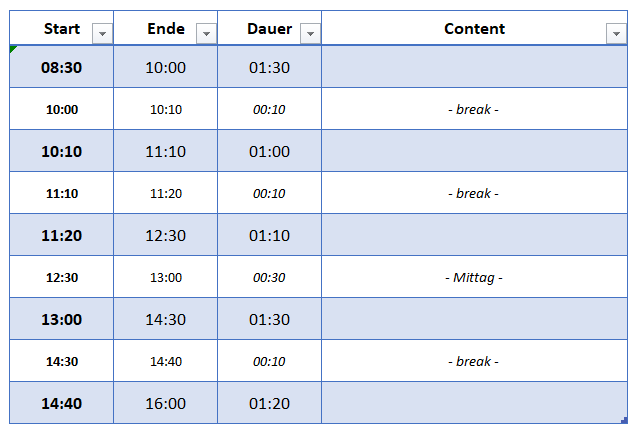
\includegraphics{assets/x.png}}

Alternativ

\hypertarget{google-konto}{%
\section{Google Konto}\label{google-konto}}

Sie brauchen ein Google-Konto für die Nutzung von Colab und ggf. für das Laden von Dateien von Google Drive.

\hypertarget{colab}{%
\section{Colab}\label{colab}}

Für unsere praktischen Aktivitäten nutzen wir die \href{https://colab.research.google.com/}{Colab-Notebooks}.

\hypertarget{programmierkenntnisse}{%
\section{Programmierkenntnisse}\label{programmierkenntnisse}}

Programmierkenntnisse sind nicht erforderlich. Sie werden das Nötige im Kurs lernen.

\hypertarget{mathematik}{%
\section{Mathematik}\label{mathematik}}

Wir benötigen folgende Grundlagen, die ich aber kurz wiederholen werde:

\begin{itemize}
\tightlist
\item
  Verteilung, Gleichverteilung, Normalverteilung, Erwartungswert, Standardabweichung, Modus, Median
\item
  Vektor, Matrix, Skalarprodukt
\item
  Funktionen, speziell lineare Abbildungen
\end{itemize}

\hypertarget{teaching-flow-agenda}{%
\section{Teaching-Flow \& Agenda}\label{teaching-flow-agenda}}

Wir springen etwas zwischen den Kapiteln, um die inhaltlichen Kapitel (A,B) nicht mit den Phython-Grundlagen (C) zu vermischen.

Link zu den in der jeweiligen Terminen erzeugten \href{https://github.com/Prof-Greipl/dsml-duf}{Colab-Notebooks}

\hypertarget{max-2000-uhr-fragen-zur-pruxfcfung}{%
\subsection{10.01.2022, 18:30 - max 20:00 Uhr: Fragen zur Prüfung}\label{max-2000-uhr-fragen-zur-pruxfcfung}}

Link: \url{https://haw-landshut-de.zoom.us/j/86239229907?pwd=eFNTUEdCeVhyMGJaaEg2YlhUdzhXdz09}

\hypertarget{uhr}{%
\subsection*{18.12.2021, 08:30 - 16:00 Uhr}\label{uhr}}
\addcontentsline{toc}{subsection}{18.12.2021, 08:30 - 16:00 Uhr}

\begin{figure}
\centering
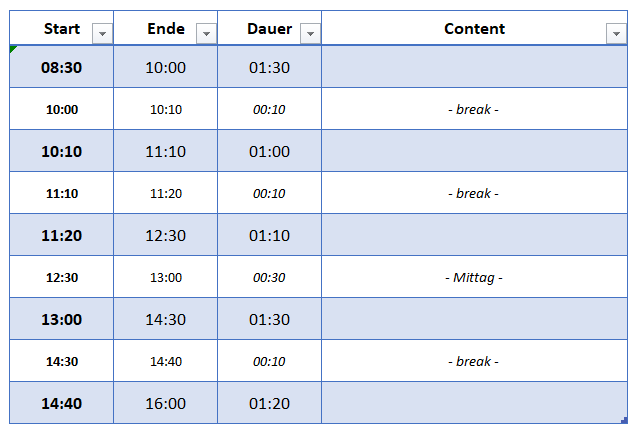
\includegraphics{assets/README.assets/image-20211218081837145.png}
\caption{image-20211218081837145}
\end{figure}

\hypertarget{uhr-1}{%
\subsection*{17.12.2021, 16:00 - 20:15 Uhr}\label{uhr-1}}
\addcontentsline{toc}{subsection}{17.12.2021, 16:00 - 20:15 Uhr}

\href{https://the-technology-lab.gitbook.io/dsml-master-duf/S0aldZCOg4S1HudPOP87/ml/0c_decision_trees}{B.2 Entscheidungsbäume - DSA Master DUF}

\href{https://the-technology-lab.gitbook.io/dsml-master-duf/S0aldZCOg4S1HudPOP87/ml/0c_train_test_val}{B.3 Training, Test und Validation - DSA Master DUF}

\href{https://the-technology-lab.gitbook.io/dsml-master-duf/S0aldZCOg4S1HudPOP87/ml/0c_regression}{B.4 Regression (und Grillen) - DSA Master DUF}

\begin{figure}
\centering
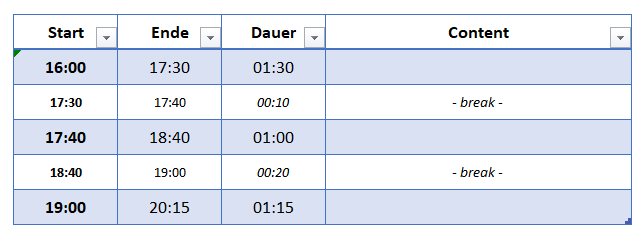
\includegraphics{assets/README.assets/image-20211217083343363.png}
\caption{image-20211217083343363}
\end{figure}

\hypertarget{uhr-2}{%
\subsection*{11.12.2021, 13:00 - 17:30 Uhr}\label{uhr-2}}
\addcontentsline{toc}{subsection}{11.12.2021, 13:00 - 17:30 Uhr}

\href{https://the-technology-lab.gitbook.io/dsml-master-duf/S0aldZCOg4S1HudPOP87/py/numpy\#elementweise-operationen}{C2. Elementweise Operationen} und \href{https://the-technology-lab.gitbook.io/dsml-master-duf/S0aldZCOg4S1HudPOP87/py/numpy\#matrix}{C.2 Numpy - Matrix}

\href{https://the-technology-lab.gitbook.io/dsml-master-duf/S0aldZCOg4S1HudPOP87/py/pandas-und-dataframes}{C.3 Pandas und Dataframes}

\href{https://the-technology-lab.gitbook.io/dsml-master-duf/S0aldZCOg4S1HudPOP87/da/0a4_visualisierung\#plots-fuer-iris}{A.2 Plots für Iris abschließen}

\href{https://the-technology-lab.gitbook.io/dsml-master-duf/S0aldZCOg4S1HudPOP87/da/0a3_preprocessing/4-datentransformation}{A.3 Preprocessing}

\href{https://the-technology-lab.gitbook.io/dsml-master-duf/S0aldZCOg4S1HudPOP87/ml/0c_ml_grundbegriffe}{B1. Problemstellung und Grundbegriffe}

\begin{figure}
\centering
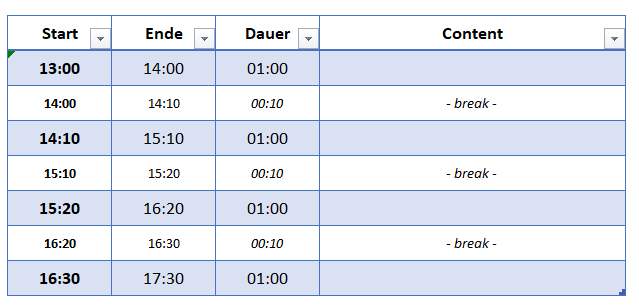
\includegraphics{assets/README.assets/image-20211211090727800.png}
\caption{image-20211211090727800}
\end{figure}

\hypertarget{uhr-3}{%
\subsection*{10.12.2012, 14:00 - 20:15 Uhr}\label{uhr-3}}
\addcontentsline{toc}{subsection}{10.12.2012, 14:00 - 20:15 Uhr}

\textbf{A.1 Datensätze}

C.1 Python - Variablen und Datentypen

C.2 Python - Numpy (ohne Matrix)

\textbf{A.2 Visualisierung} (ohne ``Bilder'', Plots für Iris noch abschließen)

\textbf{A.3 Preprocessing}

\begin{figure}
\centering
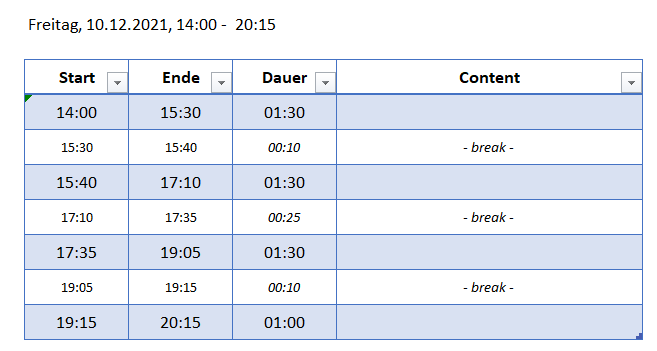
\includegraphics{assets/README.assets/image-20211210130419842.png}
\caption{image-20211210130419842}
\end{figure}

\hypertarget{hello-bookdown}{%
\chapter{Hello bookdown}\label{hello-bookdown}}

All chapters start with a first-level heading followed by your chapter title, like the line above. There should be only one first-level heading (\texttt{\#}) per .Rmd file.

\hypertarget{a-section}{%
\section{A section}\label{a-section}}

All chapter sections start with a second-level (\texttt{\#\#}) or higher heading followed by your section title, like the sections above and below here. You can have as many as you want within a chapter.

\hypertarget{an-unnumbered-section}{%
\subsection*{An unnumbered section}\label{an-unnumbered-section}}
\addcontentsline{toc}{subsection}{An unnumbered section}

Chapters and sections are numbered by default. To un-number a heading, add a \texttt{\{.unnumbered\}} or the shorter \texttt{\{-\}} at the end of the heading, like in this section.

\hypertarget{cross}{%
\chapter{Cross-references}\label{cross}}

Cross-references make it easier for your readers to find and link to elements in your book.

\hypertarget{chapters-and-sub-chapters}{%
\section{Chapters and sub-chapters}\label{chapters-and-sub-chapters}}

There are two steps to cross-reference any heading:

\begin{enumerate}
\def\labelenumi{\arabic{enumi}.}
\tightlist
\item
  Label the heading: \texttt{\#\ Hello\ world\ \{\#nice-label\}}.

  \begin{itemize}
  \tightlist
  \item
    Leave the label off if you like the automated heading generated based on your heading title: for example, \texttt{\#\ Hello\ world} = \texttt{\#\ Hello\ world\ \{\#hello-world\}}.
  \item
    To label an un-numbered heading, use: \texttt{\#\ Hello\ world\ \{-\#nice-label\}} or \texttt{\{\#\ Hello\ world\ .unnumbered\}}.
  \end{itemize}
\item
  Next, reference the labeled heading anywhere in the text using \texttt{\textbackslash{}@ref(nice-label)}; for example, please see Chapter \ref{cross}.

  \begin{itemize}
  \tightlist
  \item
    If you prefer text as the link instead of a numbered reference use: \protect\hyperlink{cross}{any text you want can go here}.
  \end{itemize}
\end{enumerate}

\hypertarget{captioned-figures-and-tables}{%
\section{Captioned figures and tables}\label{captioned-figures-and-tables}}

Figures and tables \emph{with captions} can also be cross-referenced from elsewhere in your book using \texttt{\textbackslash{}@ref(fig:chunk-label)} and \texttt{\textbackslash{}@ref(tab:chunk-label)}, respectively.

See Figure \ref{fig:nice-fig}.

\begin{Shaded}
\begin{Highlighting}[]
\FunctionTok{par}\NormalTok{(}\AttributeTok{mar =} \FunctionTok{c}\NormalTok{(}\DecValTok{4}\NormalTok{, }\DecValTok{4}\NormalTok{, .}\DecValTok{1}\NormalTok{, .}\DecValTok{1}\NormalTok{))}
\FunctionTok{plot}\NormalTok{(pressure, }\AttributeTok{type =} \StringTok{\textquotesingle{}b\textquotesingle{}}\NormalTok{, }\AttributeTok{pch =} \DecValTok{19}\NormalTok{)}
\end{Highlighting}
\end{Shaded}

\begin{figure}

{\centering 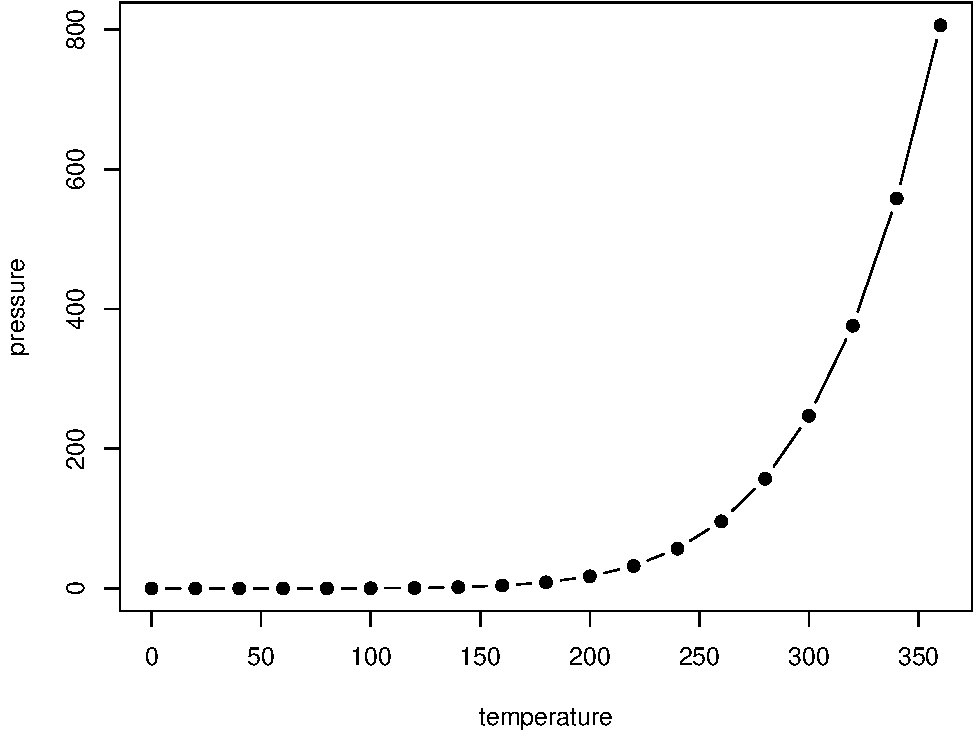
\includegraphics[width=0.8\linewidth]{02-cross-refs_files/figure-latex/nice-fig-1} 

}

\caption{Here is a nice figure!}\label{fig:nice-fig}
\end{figure}

Don't miss Table \ref{tab:nice-tab}.

\begin{Shaded}
\begin{Highlighting}[]
\NormalTok{knitr}\SpecialCharTok{::}\FunctionTok{kable}\NormalTok{(}
  \FunctionTok{head}\NormalTok{(pressure, }\DecValTok{10}\NormalTok{), }\AttributeTok{caption =} \StringTok{\textquotesingle{}Here is a nice table!\textquotesingle{}}\NormalTok{,}
  \AttributeTok{booktabs =} \ConstantTok{TRUE}
\NormalTok{)}
\end{Highlighting}
\end{Shaded}

\begin{table}

\caption{\label{tab:nice-tab}Here is a nice table!}
\centering
\begin{tabular}[t]{rr}
\toprule
temperature & pressure\\
\midrule
0 & 0.0002\\
20 & 0.0012\\
40 & 0.0060\\
60 & 0.0300\\
80 & 0.0900\\
\addlinespace
100 & 0.2700\\
120 & 0.7500\\
140 & 1.8500\\
160 & 4.2000\\
180 & 8.8000\\
\bottomrule
\end{tabular}
\end{table}

\hypertarget{parts}{%
\chapter{Parts}\label{parts}}

You can add parts to organize one or more book chapters together. Parts can be inserted at the top of an .Rmd file, before the first-level chapter heading in that same file.

Add a numbered part: \texttt{\#\ (PART)\ Act\ one\ \{-\}} (followed by \texttt{\#\ A\ chapter})

Add an unnumbered part: \texttt{\#\ (PART\textbackslash{}*)\ Act\ one\ \{-\}} (followed by \texttt{\#\ A\ chapter})

Add an appendix as a special kind of un-numbered part: \texttt{\#\ (APPENDIX)\ Other\ stuff\ \{-\}} (followed by \texttt{\#\ A\ chapter}). Chapters in an appendix are prepended with letters instead of numbers.

\hypertarget{footnotes-and-citations}{%
\chapter{Footnotes and citations}\label{footnotes-and-citations}}

\hypertarget{footnotes}{%
\section{Footnotes}\label{footnotes}}

Footnotes are put inside the square brackets after a caret \texttt{\^{}{[}{]}}. Like this one \footnote{This is a footnote.}.

\hypertarget{citations}{%
\section{Citations}\label{citations}}

Reference items in your bibliography file(s) using \texttt{@key}.

For example, we are using the \textbf{bookdown} package \citep{R-bookdown} (check out the last code chunk in index.Rmd to see how this citation key was added) in this sample book, which was built on top of R Markdown and \textbf{knitr} \citep{xie2015} (this citation was added manually in an external file book.bib).
Note that the \texttt{.bib} files need to be listed in the index.Rmd with the YAML \texttt{bibliography} key.

The \texttt{bs4\_book} theme makes footnotes appear inline when you click on them. In this example book, we added \texttt{csl:\ chicago-fullnote-bibliography.csl} to the \texttt{index.Rmd} YAML, and include the \texttt{.csl} file. To download a new style, we recommend: \url{https://www.zotero.org/styles/}

The RStudio Visual Markdown Editor can also make it easier to insert citations: \url{https://rstudio.github.io/visual-markdown-editing/\#/citations}

\hypertarget{blocks}{%
\chapter{Blocks}\label{blocks}}

\hypertarget{equations}{%
\section{Equations}\label{equations}}

Here is an equation.

\begin{equation} 
  f\left(k\right) = \binom{n}{k} p^k\left(1-p\right)^{n-k}
  \label{eq:binom}
\end{equation}

You may refer to using \texttt{\textbackslash{}@ref(eq:binom)}, like see Equation \eqref{eq:binom}.

\hypertarget{theorems-and-proofs}{%
\section{Theorems and proofs}\label{theorems-and-proofs}}

Labeled theorems can be referenced in text using \texttt{\textbackslash{}@ref(thm:tri)}, for example, check out this smart theorem \ref{thm:tri}.

\begin{theorem}
\protect\hypertarget{thm:tri}{}\label{thm:tri}For a right triangle, if \(c\) denotes the \emph{length} of the hypotenuse
and \(a\) and \(b\) denote the lengths of the \textbf{other} two sides, we have
\[a^2 + b^2 = c^2\]
\end{theorem}

Read more here \url{https://bookdown.org/yihui/bookdown/markdown-extensions-by-bookdown.html}.

\hypertarget{callout-blocks}{%
\section{Callout blocks}\label{callout-blocks}}

The \texttt{bs4\_book} theme also includes special callout blocks, like this \texttt{.rmdnote}.

You can use \textbf{markdown} inside a block.

\begin{Shaded}
\begin{Highlighting}[]
\FunctionTok{head}\NormalTok{(beaver1, }\AttributeTok{n =} \DecValTok{5}\NormalTok{)}
\CommentTok{\#\textgreater{}   day time  temp activ}
\CommentTok{\#\textgreater{} 1 346  840 36.33     0}
\CommentTok{\#\textgreater{} 2 346  850 36.34     0}
\CommentTok{\#\textgreater{} 3 346  900 36.35     0}
\CommentTok{\#\textgreater{} 4 346  910 36.42     0}
\CommentTok{\#\textgreater{} 5 346  920 36.55     0}
\end{Highlighting}
\end{Shaded}

It is up to the user to define the appearance of these blocks for LaTeX output.

You may also use: \texttt{.rmdcaution}, \texttt{.rmdimportant}, \texttt{.rmdtip}, or \texttt{.rmdwarning} as the block name.

The R Markdown Cookbook provides more help on how to use custom blocks to design your own callouts: \url{https://bookdown.org/yihui/rmarkdown-cookbook/custom-blocks.html}

\hypertarget{sharing-your-book}{%
\chapter{Sharing your book}\label{sharing-your-book}}

\hypertarget{publishing}{%
\section{Publishing}\label{publishing}}

HTML books can be published online, see: \url{https://bookdown.org/yihui/bookdown/publishing.html}

\hypertarget{pages}{%
\section{404 pages}\label{pages}}

By default, users will be directed to a 404 page if they try to access a webpage that cannot be found. If you'd like to customize your 404 page instead of using the default, you may add either a \texttt{\_404.Rmd} or \texttt{\_404.md} file to your project root and use code and/or Markdown syntax.

\hypertarget{metadata-for-sharing}{%
\section{Metadata for sharing}\label{metadata-for-sharing}}

Bookdown HTML books will provide HTML metadata for social sharing on platforms like Twitter, Facebook, and LinkedIn, using information you provide in the \texttt{index.Rmd} YAML. To setup, set the \texttt{url} for your book and the path to your \texttt{cover-image} file. Your book's \texttt{title} and \texttt{description} are also used.

This \texttt{bs4\_book} provides enhanced metadata for social sharing, so that each chapter shared will have a unique description, auto-generated based on the content.

Specify your book's source repository on GitHub as the \texttt{repo} in the \texttt{\_output.yml} file, which allows users to view each chapter's source file or suggest an edit. Read more about the features of this output format here:

\url{https://pkgs.rstudio.com/bookdown/reference/bs4_book.html}

Or use:

\begin{Shaded}
\begin{Highlighting}[]
\NormalTok{?bookdown}\SpecialCharTok{::}\NormalTok{bs4\_book}
\end{Highlighting}
\end{Shaded}


  \bibliography{book.bib,packages.bib}

\end{document}
